\documentclass[final]{beamer}

% ====================
% Packages
% ====================

\usepackage[T1]{fontenc}
 \usepackage[utf8]{luainputenc}
\usepackage{lmodern}
\usepackage[size=custom,width=297,height=210,scale=3.2]{beamerposter} % A4: 297mm x 210mm
\usetheme{gemini}
\usecolortheme{utb}
\usepackage{graphicx}
\usepackage{booktabs}
\usepackage{tikz}
\usepackage{pgfplots}
\pgfplotsset{compat=1.14}
\usepackage{anyfontsize}

% ====================
% Lengths
% ====================

% If you have N columns, choose \sepwidth and \colwidth such that
% (N+1)*\sepwidth + N*\colwidth = \paperwidth
\newlength{\sepwidth}
\newlength{\colwidth}
\setlength{\sepwidth}{0.025\paperwidth}
\setlength{\colwidth}{0.3\paperwidth}

\newcommand{\separatorcolumn}{\begin{column}{\sepwidth}\end{column}}

% ====================
% Title
% ====================

\title{\resizebox{\textwidth}{!}{Automatic Assessment of Tasks in the Course Programming Network Applications}}

\author{\textbf{Author: Ing. Martin Krčma}, Supervisor: Ing. Tomáš Dulík, Ph.D.}

\institute[shortinst]{\textbf{Tomas Bata University in Zlin - Faculty of Applied Informatics}} 

% ====================
% Footer (optional)
% ====================

\footercontent{
  \href{https://github.com/0xMartin}{Github: \textbf{https://github.com/0xMartin}} 
  \hfill
  \href{https://github.com/0xMartin/NetworkAppTestingTool}{Project repository: \textbf{https://github.com/0xMartin/NetworkAppTestingTool}} 
  }
% (can be left out to remove footer)

% ====================
% Logo (optional)
% ====================

% use this to include logos on the left and/or right side of the header:
% Left: institution
 \logoright{
\includegraphics[height=12cm]{imgs/FAI_ico.png}}
% Right: funding agencies and other affilations 
%\logoright{\includegraphics[height=7cm]{logos/NSF.eps}}
% ====================
% Body
% ====================

\begin{document}



\begin{frame}[t]
\begin{columns}[t]
\separatorcolumn

\begin{column}{\colwidth}

  \begin{block}{1. Motivation}

    The primary motivation for this thesis was to solve the problem associated with the \textbf{increasing
    number of students at the faculty} and to ease the workload of teachers in evaluating tasks.
    This work specifically focuses on the programming network applications course, where verifying
    the functionality of students' solutions often requires additional network resources (servers, clients, ...),
    making the assessment process time-consuming. Network applications \textbf{often have varied behaviors
    and communicate in different ways}, which poses a significant challenge in creating a 
    universal solution that can accommodate all these testing needs.

    \hspace{2em}Therefore, the goal was to develop a flexible, universal and easy solution that would
    allow the testing of software \textbf{locally and within GitLab repositories}, without
    relying on external network resources. This will help students and, more importantly, teachers,
    as this solution will save them a significant amount of time, allowing them to focus on more
    important matters at the faculty. This solution is not limited to educational institutions,
    it can also be used in a wide range of software projects.
  
  \end{block}

  \begin{block}{2. Conclusion}

    The result of this thesis is a \textbf{universal black-box testing tool} that effectively enables the testing
    of network applications. This tool, developed in Java and designed to be cross-platform, supports 
    testing across a wide range of network applications using commonly employed communication protocols.
    It is easily \textbf{configurable via YAML}, and a straightforward configuration language has been created 
    to define test scenarios using a basic set of keywords. Additionally, a \textbf{simple IDE} was developed to
    facilitate the creation and runtime testing of these test scenario configurations.

    \hspace{2em}This thesis includes not only the the \textbf{Network Application Testing Tool (NATT)} but also the 
    \textbf{Configuration Editor}, documentation for tool, example projects and configurations, a new set consisting of 8 tasks 
    for a network programming course, GitLab repositories for each task and aditional tools for course.

    \begin{figure}
      \centering
        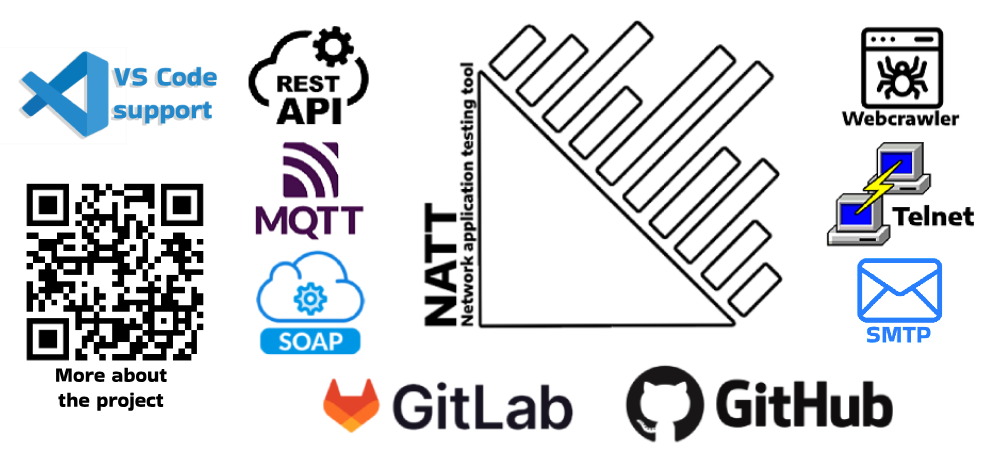
\includegraphics[width=1.0\textwidth]{./imgs/natt-main-banner.png}
      \caption{Network Application Testing Tool (NATT) - supported technologies} 
    \end{figure}

  \end{block}

\end{column}

\separatorcolumn

\begin{column}{\colwidth}

  \begin{alertblock}{3. Main features of testing tool}

    This Black Box Testing Tool automates the testing and evaluation of software 
    applications without needing internal implementation details. It supports a 
    \textbf{wide range} of applications, operates \textbf{independently of external network resources} 
    by creating virtual servers and clients, and offers flexible configuration for 
    defining new test scenarios.

    \heading{What does the tool allow you to test?}
    \begin{enumerate}
      \item Testing simple \textbf{email} sending applications
      \item Testing \textbf{clients} that use the telnet protocol
      \item Testing \textbf{servers} that use the telnet protocol
      \item Testing applications that use \textbf{REST API}
      \item Testing \textbf{SOAP web services}
      \item Testing \textbf{MQTT clients}
      \item Testing \textbf{Web crawlers}
      \item Testing the application through the \textbf{standard stream}
    \end{enumerate}

  \end{alertblock}

  \begin{block}{4. Principle of the testing tool}

    These two diagrams illustrate how application testing is conducted using the \textbf{NATT}
    black box testing tool. The diagrams show the process of \textbf{how the tool interacts} 
    with different types of applications. 

    \hspace{2em} On the left side of each diagram, the testing tool communicates with 
    the tested application through \textbf{virtually created modules (highlighted in blue)}. This 
    communication is then evaluated to determine if the application meets the defined
    expectations.

    \begin{figure}
      \centering
        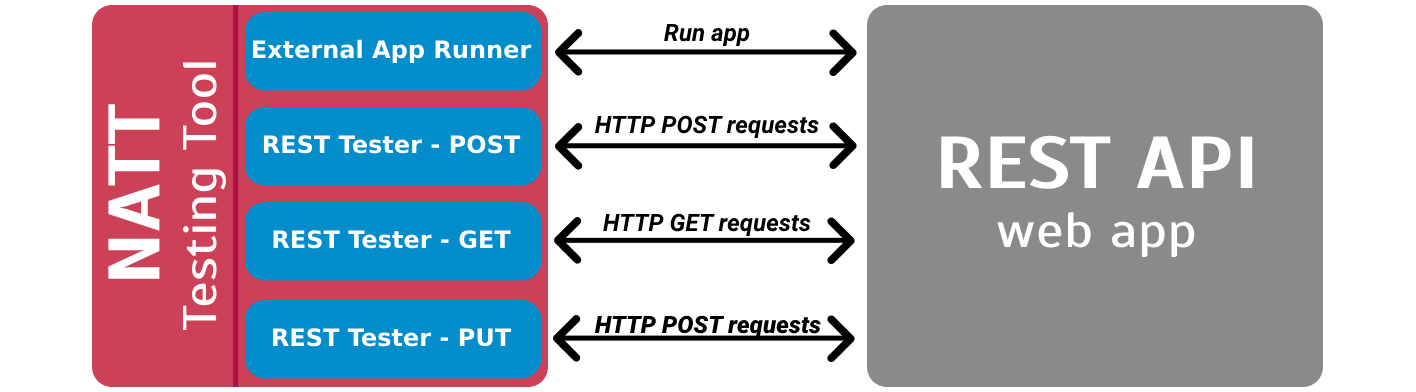
\includegraphics[width=1.0\textwidth]{./imgs/simple-rest-diagram.png}
      \caption{Testing of REST API application}
    \end{figure}

    \begin{figure}
      \centering
        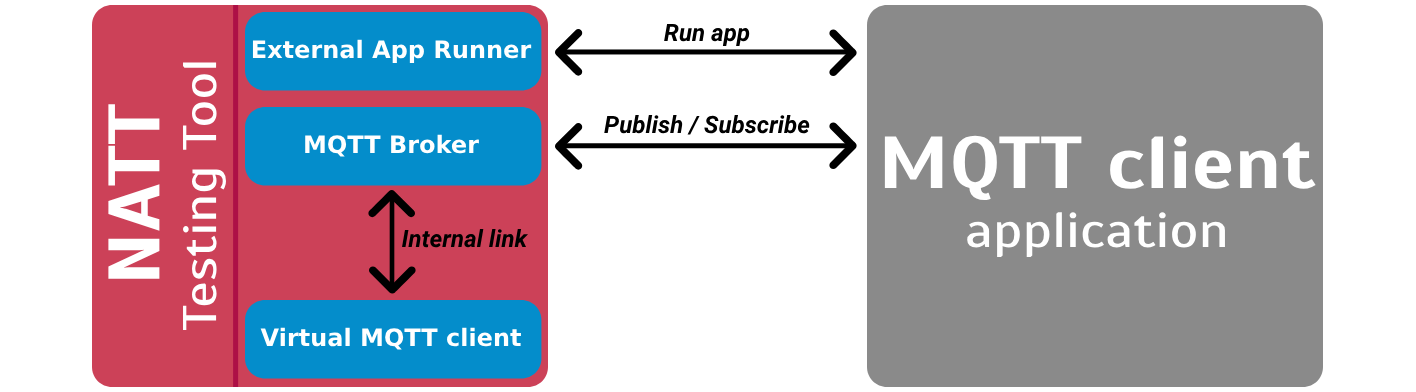
\includegraphics[width=1.0\textwidth]{./imgs/simple-mqtt-diagram.png}
      \caption{Testing of MQTT application}
    \end{figure}

  \end{block}

\end{column}

\separatorcolumn

\begin{column}{\colwidth}

  \begin{block}{5. Test scenarios and configuration}

    The image below illustrates how test scenarios are defined for this tool. At the 
    beginning is the Test Root node, which is the \textbf{entry point} for each test 
    scenario configuration. This root node sets the overall context for the testing 
    process and encompasses all test suites within it. 

    \hspace{2em} The diagram illustrates the \textbf{context of each test segment} and the 
    duration for which variables or resources remain active. On the right side, a simplified
    test scenario configuration is shown, which NATT \textbf{uses to generate} an acyclic graph that 
    is subsequently executed.

    \begin{figure}
      \centering
        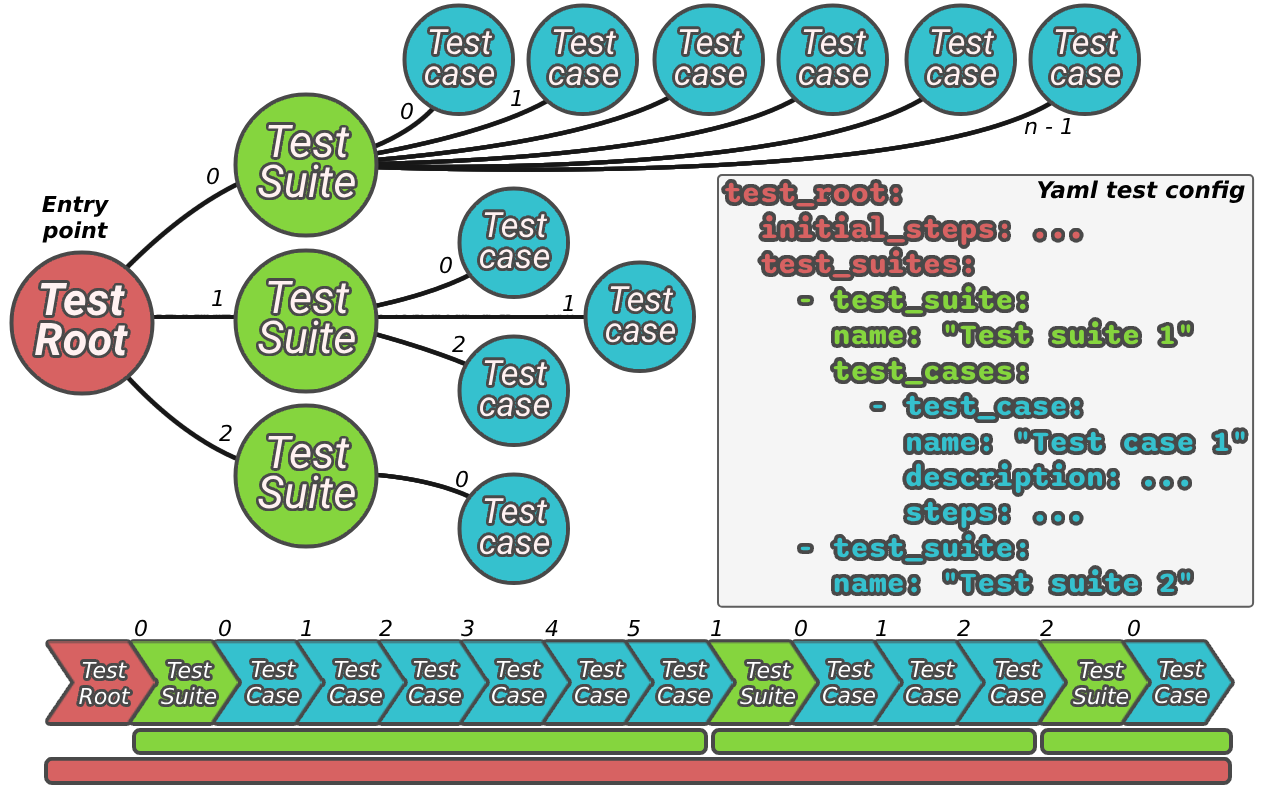
\includegraphics[width=1.0\textwidth]{./imgs/test-config-struct.png}
      \caption{Testing structure and configuration}
    \end{figure}

  \end{block}

  \begin{exampleblock}{6. Usage of testing tool}

    \begin{enumerate}
      \item \textbf{Educational Use:} Automates and standardizes student assignment evaluations in network programming courses.
      
      \item \textbf{Professional Use:} Facilitates efficient testing and debugging of network applications in software development.
      
      \item \textbf{Programming Competitions:} Provides automated testing and fair evaluation for multiple submissions in competitive programming events.
   \end{enumerate}
 
  \end{exampleblock}

  \begin{block}{7. NATT Config Editor \& VS Code Extension}

    \begin{minipage}{0.7\textwidth}
      NATT config Editor is simple IDE and offers an easy interface for \textbf{creating test configurations}. It includes an 
      \textbf{auto-completion} feature, \textbf{running} the test scenario and viewing of the final test report. For NATT is 
      also available an \textbf{extension for VS Code}, which allows the same functions as the mentioned editor.
    \end{minipage}
    \hfill
    \noindent\begin{minipage}{0.25\textwidth}
      
\includegraphics[width=\textwidth]{./imgs/extension_qr.png}
    \end{minipage}

  \end{block}

\end{column}

\separatorcolumn
\end{columns}
\end{frame}

\end{document}
